%! Author = taj
%! Date = 7/22/25

% Preamble
\documentclass[11pt]{article}

% Packages
\usepackage{amsmath}
\usepackage{graphicx}
\usepackage{float}
\usepackage{upgreek}

\title{11. Statično ravnovesje: Biomehanika človeške roke}
\author{Taj Šobot}

% Document
\begin{document}
    \maketitle
    \flushleft
    Pri tej vaji smo opazovali in računali navore v modelu človeške roke.

    Skica eksperimenta (model roke):
    \begin{figure}[H]
        \centering
        
\includegraphics[width=0.9\textwidth]{img}
        \caption{Skica eksperimenta: Model roke}
        \label{fig:1}
    \end{figure}

    \section{Meritve}
    Obravnava sil, ki delujejo na sistem.
    \begin{figure}[H]
        \centering
        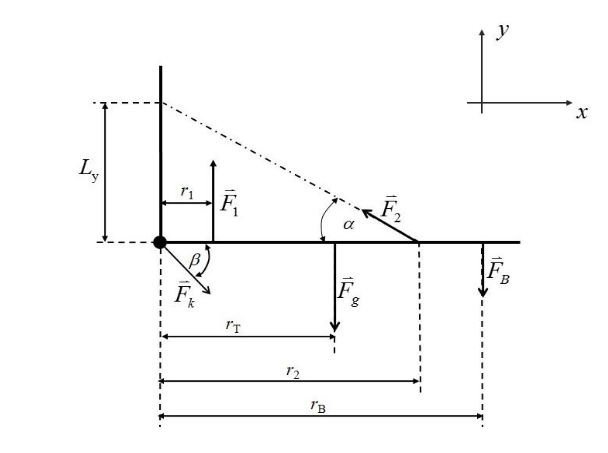
\includegraphics[width=0.9\textwidth]{img2}
        \caption{Obravnava sil}
        \label{fig:2}
    \end{figure}
    Meritve raznih razdalji:
    \begin{align*}
        r_1 = (4.8 \pm 0.1) cm \\
        r_2 = (27.5 \pm 0.1) cm\\
        r_{cele} = (48.1 \pm 0.1) \\
        r_B = (40.7 \pm 1) cm \\
        r_T = \frac{1}{2} r_{cele} \\
        L_y = (4.2 \pm 0.1) cm
    \end{align*}
    Izmerili smo tudi maso podlahti (za $F_g$):
    \[
        m_{podlaht} = (50 \pm 1) g
    \]

    \section{Rezultati}
    \subsection{Poenostavljen primer}
    Prvo smo obravnavali enostavnejši primer samo z eno "mišico" ($f_1$ na skici).
    Izračunali smo:
    \[
        F_g = m_p g = (0.89 \pm 0.01)N
    \]
    Dinamometer je odčital(enkrat smo vsilili vodoravno lego):
    \begin{align*}
        F_{1v} = (2.4 \pm 0.2)N \\
        F_{1} = (2.8 \pm 0.2)N \\
    \end{align*}

    nato pa smo uporabili oba dinamometra (2 "mišici"):
    \begin{align*}
        F_{1} = (2.0 \pm 0.2)N \\
        F_{2} = (2.8 \pm 0.2)N \\
    \end{align*}
    Iz pogoja za ravnovesje izpeljemo :
    \\
    X smer:
    \begin{align*}
        F_{kx} - F_2 \cos(\alpha) = 0 \\
        \alpha = \tan^{-1} (\frac{L_y}{r_2})
    \end{align*}
    Vstavimo:
    \[
        F_{kx} = (2.1 \pm 0.4) N
    \]
    Še Y smer:
    \begin{align*}
        F_1 + F_2 \sin(\alpha) - F_g - F_{ky} = 0 \\
        F_{ky} = F_1 + f_2 \sin(\alpha) - F_g
    \end{align*}
    Vstavimo:
    \[
        F_{ky} = (2.9 \pm 0.4) N
    \]
    Pitagora in dobimo:
    \[
        F_k = \sqrt[2]{F_{ky}^2 + f_{kx}^2} = (3.6 \pm 0.3) N
    \]
    Zdaj lahko še izračunamo kot $\beta$:
    \[
        \beta = \tan^{-1} (\frac{F_ky}{F_kx}) = (54.1 \pm 7) ^\circ
    \]
    Preverimo še pogoj za ravnovesje navorov:
    \[
        F_1 r_1 - F_g r_T + F_2 r_2 \sin(\alpha) - F_B r_B = 0
    \]
    Ko vstavimo dobimo vrednost:
    \[
        (-0.18 \pm 0.05) Nm \neq 0
    \]
    Rezultat je blizu... Ampak ni znotraj napake.
    \section{Odgovori na vprašanja}

    1.a) Na skico narisana sila...

    \begin{figure}[H]
        \centering
        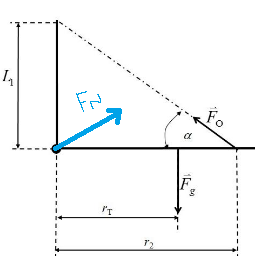
\includegraphics[width=0.9\textwidth]{img3}
        \caption{vprašanje 1}
        \label{fig:3}
    \end{figure}
    Da roka ostane v ravnovesju more ta sila delovati malo navzgor in v desno.
    \\

    1.c) Silo $F_{0y} = F_g$

\end{document}